\documentclass[12pt,a4paper]{article}

\usepackage{graphicx}
\usepackage[left=2cm,right=2cm,top=2cm,bottom=2cm]{geometry}
\usepackage{listings}
\usepackage{lstlang-go}
% Copyright 2017 Sergei Tikhomirov, MIT License
% https://github.com/s-tikhomirov/solidity-latex-highlighting/

\usepackage{listings, xcolor}

\definecolor{verylightgray}{rgb}{.97,.97,.97}

\lstdefinelanguage{Solidity}{
	keywords=[1]{anonymous, assembly, assert, balance, break, call, callcode, case, catch, class, constant, continue, constructor, contract, debugger, default, delegatecall, delete, do, else, emit, event, experimental, export, external, false, finally, for, function, gas, if, implements, import, in, indexed, instanceof, interface, internal, is, length, library, log0, log1, log2, log3, log4, memory, modifier, new, payable, pragma, private, protected, public, pure, push, require, return, returns, revert, selfdestruct, send, solidity, storage, struct, suicide, super, switch, then, this, throw, transfer, true, try, typeof, using, value, view, while, with, addmod, ecrecover, keccak256, mulmod, ripemd160, sha256, sha3}, % generic keywords including crypto operations
	keywordstyle=[1]\color{blue}\bfseries,
	keywords=[2]{address, bool, byte, bytes, bytes1, bytes2, bytes3, bytes4, bytes5, bytes6, bytes7, bytes8, bytes9, bytes10, bytes11, bytes12, bytes13, bytes14, bytes15, bytes16, bytes17, bytes18, bytes19, bytes20, bytes21, bytes22, bytes23, bytes24, bytes25, bytes26, bytes27, bytes28, bytes29, bytes30, bytes31, bytes32, enum, int, int8, int16, int24, int32, int40, int48, int56, int64, int72, int80, int88, int96, int104, int112, int120, int128, int136, int144, int152, int160, int168, int176, int184, int192, int200, int208, int216, int224, int232, int240, int248, int256, mapping, string, uint, uint8, uint16, uint24, uint32, uint40, uint48, uint56, uint64, uint72, uint80, uint88, uint96, uint104, uint112, uint120, uint128, uint136, uint144, uint152, uint160, uint168, uint176, uint184, uint192, uint200, uint208, uint216, uint224, uint232, uint240, uint248, uint256, var, void, ether, finney, szabo, wei, days, hours, minutes, seconds, weeks, years},	% types; money and time units
	keywordstyle=[2]\color{teal}\bfseries,
	keywords=[3]{block, blockhash, coinbase, difficulty, gaslimit, number, timestamp, msg, data, gas, sender, sig, value, now, tx, gasprice, origin},	% environment variables
	keywordstyle=[3]\color{violet}\bfseries,
	identifierstyle=\color{black},
	sensitive=false,
	comment=[l]{//},
	morecomment=[s]{/*}{*/},
	commentstyle=\color{gray}\ttfamily,
	stringstyle=\color{red}\ttfamily,
	morestring=[b]',
	morestring=[b]"
}

\lstset{
	language=Solidity,
	backgroundcolor=\color{verylightgray},
	extendedchars=true,
	basicstyle=\footnotesize\ttfamily,
	showstringspaces=false,
	showspaces=false,
	numbers=left,
	numberstyle=\footnotesize,
	numbersep=9pt,
	tabsize=2,
	breaklines=true,
	showtabs=false,
	captionpos=b
}
\usepackage{multirow}

\setlength{\parindent}{0em}

\begin{document}

\noindent
\begin{minipage}{120mm}
        {\huge {\bf School of Informatics}}\\
        {\Large {\bf Blockchains and Distributed Ledgers}}\\

        {\Large Assignment 3}\\
        {\normalsize Erodotos Demetriou (s2187344)}
\end{minipage}
\hfill
\begin{minipage}{40mm}              
        
\includegraphics[width=40mm]{crest.png}
\end{minipage}

\begin{center}
\rule{\linewidth}{0.5mm}
\end{center}

\section*{Part 1}

For Part A of this assignment we are required to interact with a smart contract
deployed on the \emph{Ethereum Ropsten network}. In more detail, we should call
the \emph{register} method, giving as input arguments a secret key and our student
number. Since \emph{Ethereum} is a public Blockchain, everything can be accessed
on chain. Hence, the following script was used to retrive the secret key from
the smart contract's storage. \\

\begin{lstlisting}
const Web3 = require('web3');

var web3 = new Web3(new Web3.providers.HttpProvider('https://ropsten.infura.io/v3/0ab1814012ad4231965d67bf98a40b1a'));

var contract_address = '0xde3a17573B0128da962698917B17079f2aAbebea';

web3.eth.getStorageAt(contract_address, 1).then(result => {
    console.log(web3.utils.hexToString(result));
});
\end{lstlisting} 

\vspace{5mm}

The found key is : \emph{actually...;)}. We imported the smart contract source
code and deployed address into remix and finally called the \emph{register}
function with input \emph{actually...;)} and \emph{s2187344} as inputs. \\

Transaction Hash : 0xc6ebbfea38258b115d07d5826667dfdd2445a5cbe277f0c3e18fa5a294ef3d32

\section*{Part 2 A}

\subsection*{Smart Contract High-Level Description}

\begin{center}
    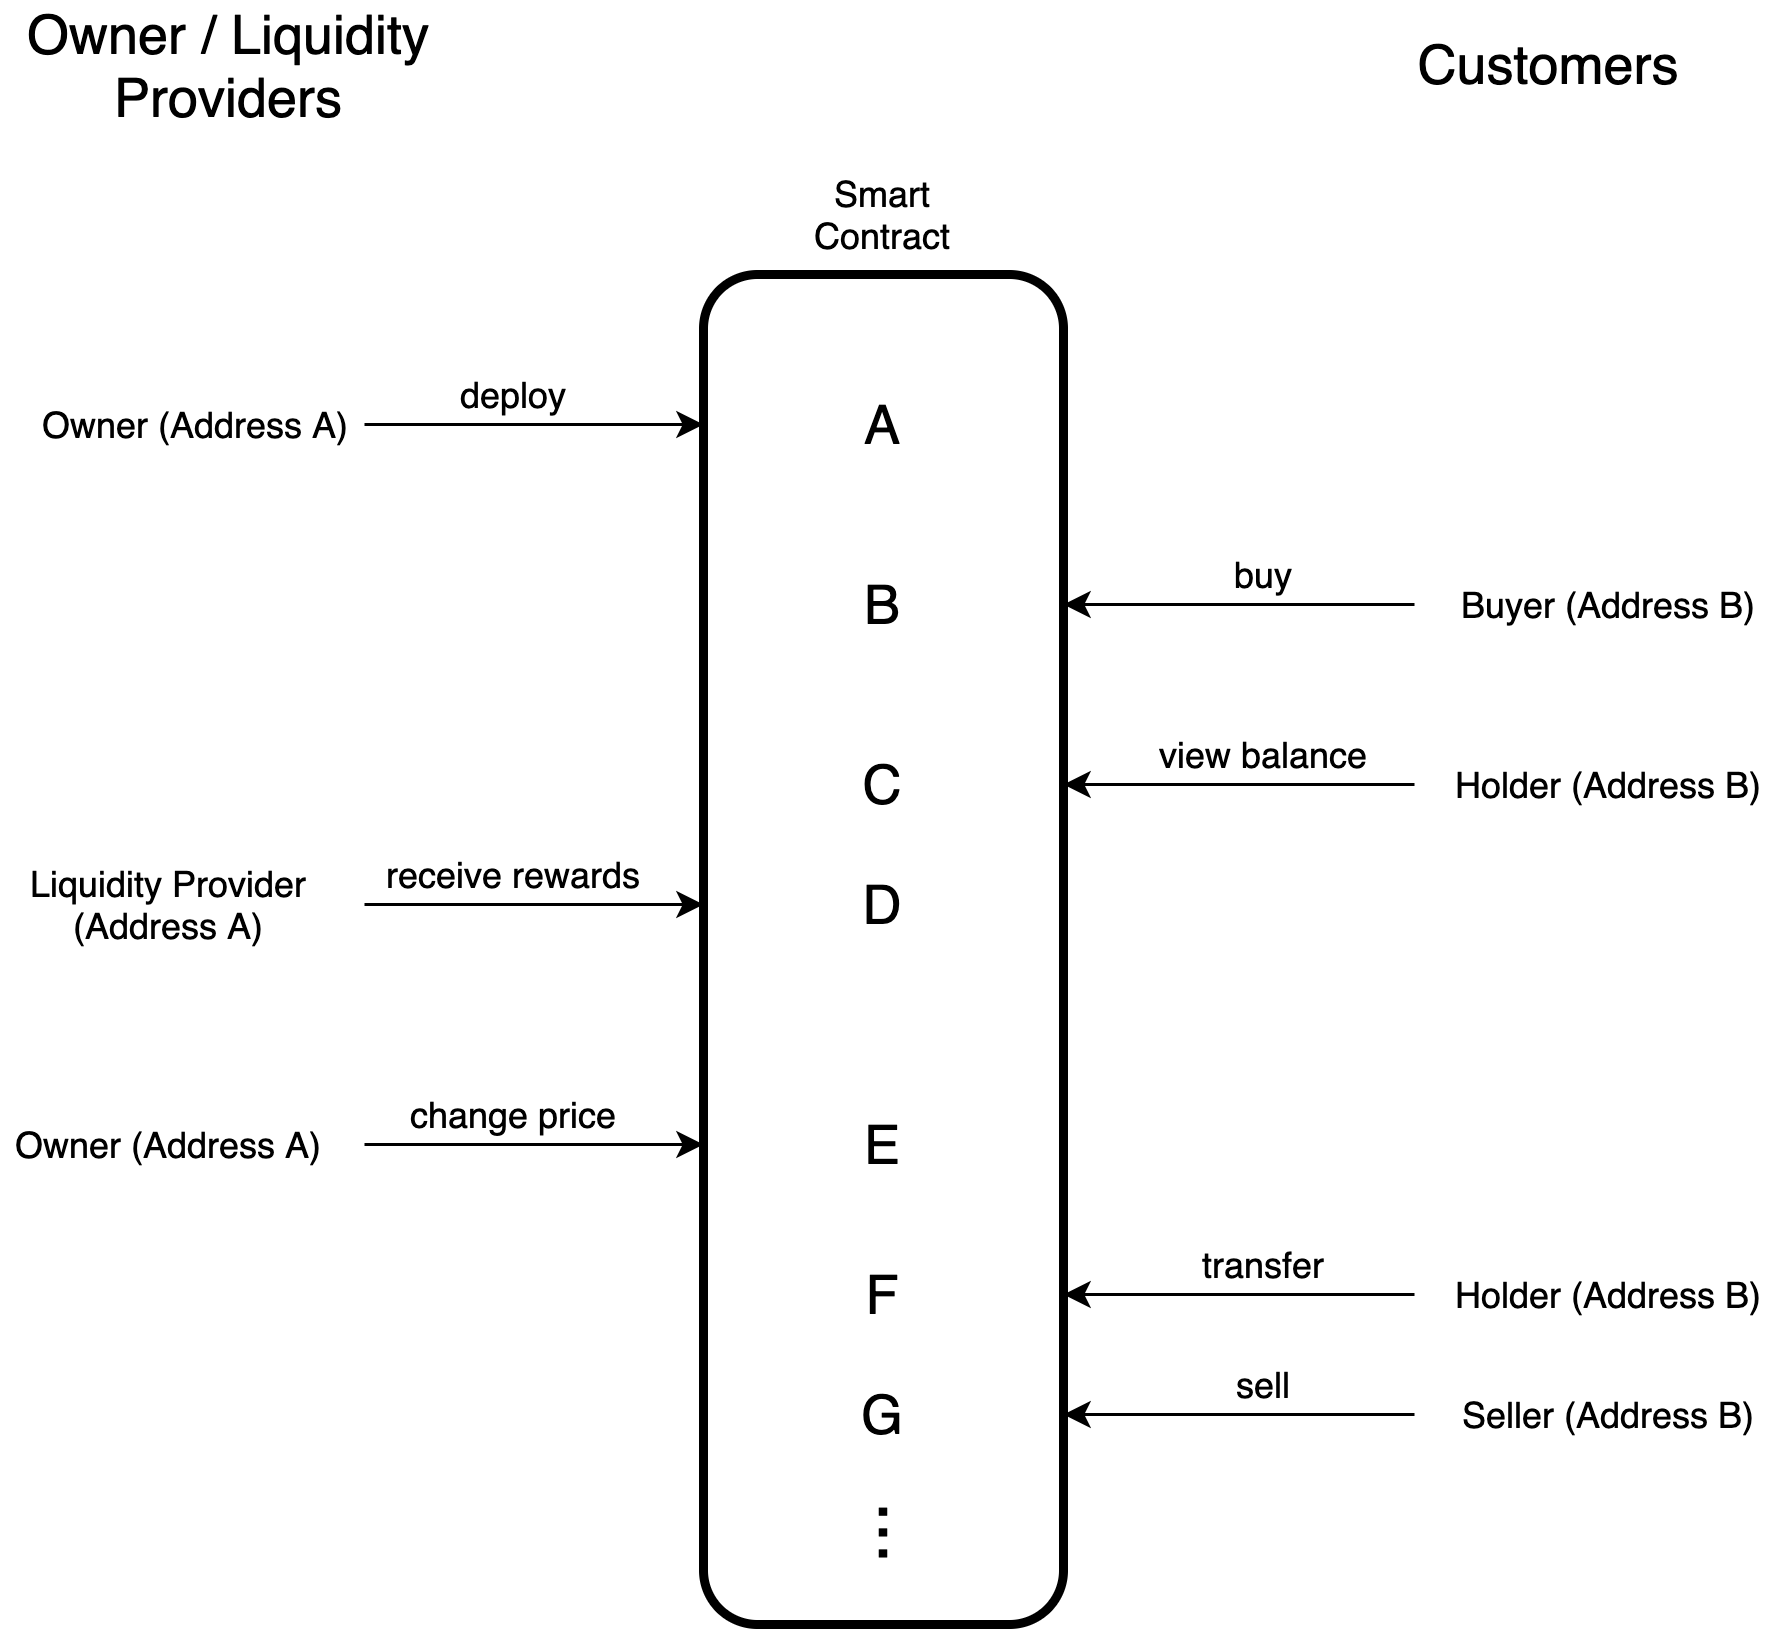
\includegraphics[height=10cm]{execution_flow.png}
\end{center}

\textbf{\underline{Variables}} \\

\emph{address owner:} This variable is set on deployment, and stores the smart
contract's owner address.\\

\emph{uint256 contractBalance:} This variable stores the number of \emph{wei} deposited
into the smart contract.\\

\emph{uint256 circulatingTokens:}  This variable stores the number of
circulating tokens.\\

\emph{mapping balances:} This is a mapping variable maintaining a one to one
correspondance between a user address and the number of tokens it holds. \\

\emph{mapping liquidityProviders:} This is a mapping variable maintaining a one
to one correspondance between a liquidity provider user address and the amount
of liquidity it provided in \emph{wei}. \\

\emph{uint256 numberOfProviders:} This variable holds the number of total
liquidity providers.\\

\emph{uint256 totalLiquidity:} This variable holds the amount of total liquidity
provided during the complete life cycle of the smart contract.\\

\emph{uint256 rewardsPool:} This variable stores the amount of tokens that will
be available to liquidity providers as rewards for their services.\\

\emph{uint256 tokenPrice:} This variable stores the current token price in
\emph{wei}.\\

\textbf{\underline{Events}} \\

\emph{event Purchase:} Whenever a token purchase is fulfilled, an event stating
the buyer's address and the purchased amount, is emitted.\\

\emph{event Sell:} Whenever a token holder sells its tokens back to the smart
contract, a sell event is emitted. This event states the seller address and the
amount of tokens sold.\\

\emph{event Transfer:} Whenever a token holder transfers its tokens to an other
address a transfer event is emitted. This event states the sender and receiver
adddresses, as well as the transfered amount of tokens.\\

\emph{event Price:} This event is emitted whenever the smart contract owner
changes the token price.\\

\textbf{\underline{Functions}} \\

\emph{constructor():} This is the smart contract constractor. It is called
whenever the code is deployed for the first time, and sets the contract owner,
as the initiator of the transaction. The smart contract constructor requirement
is that the owner provides 100 \emph{wei} as initial liquidity. Thus he becomes
the first liquidity provider.\\

\emph{buyToken():} Whenever a buyer wants to exchange his ETH for our token has
to call this function. In more detail, he needs to provide as input the number
of tokens that he desires to purchase and send the proportional amount of ETH,
considering the token price which is in \emph{wei}.\\

\emph{transfer():} This function can be called by a token holder that desires to
transfer a specific amount of tokens to an other address.\\

\emph{sellToken():} This function enables a token holder to exchange his tokens
with ETH. He can provide the number of tokens he wants to exchange and
subsequentyl he will receive the according value of ETH considering the current
token price.\\

\emph{changePrice():} This function can be called only by the smart contract
owner, to change the token price. Its execution will only succed if there is
enough liquidity to pay token holders if they decide to sell their token
simultaneously.\\

\emph{getBalance():} This function returns the balance of tokens that are in the
posetion of the fucntion's caller.\\

\emph{provideLiquidity():} This is an internal function that can be triggered
through the fallback function. It receives an address and the amount of provided
liquidity. Subsequentyl, it registers this user as a liquidity provider. \\

\emph{getReward():} This is an internal function that can be trigered through
the fallback function and only if the caller is a registered liquidity provider.
Its execution results into receiving a proportion of the reward tokens from the
reward pool.\\

\emph{fallback():} This function can be used with different arguments and can
serve different purposes. If it is called providing some ETH, registers you as a
liquidity provider; Else, it can be used by liquidity provider to receive its
rewards.\\



\subsection*{Gas Costs Evaluation}
This section measures and evaluates the gas cost we expect to have when deploying and
interacting with the Smart Contract. \\

Gas costs appear in the following table, and they are unquestionably high.
The Smart Contract owner has to pay 1,801,345 gas units to deploy the code, which is
approximately \$995 (price on 26/10/21). This is definitely a high amount of gas which makes the
Smart Contract not so gas efficient. \\

\begin{table}[htpb]
    \begin{center}
        \begin{tabular}{ccc}
        \multicolumn{3}{c}{\textbf{Gas Costs}}                                                                                                                   \\
        \multicolumn{1}{l}{}                                 & \multicolumn{1}{l}{}                            & \multicolumn{1}{l}{}                            \\ \hline
        \multicolumn{3}{|c|}{\textit{\textbf{Contract Owner Fees}}}                                                                                              \\ \hline
        \multicolumn{1}{|c|}{Contract Deployment}            & \multicolumn{2}{c|}{1,801,345}                                                                    \\ \hline
        \multicolumn{1}{l}{}                                 & \multicolumn{1}{l}{}                            & \multicolumn{1}{l}{}                            \\ \hline
        \multicolumn{1}{|c|}{\textit{\textbf{Players Fees}}} & \multicolumn{1}{c|}{\textit{\textbf{Player A}}} & \multicolumn{1}{c|}{\textit{\textbf{Player B}}} \\ \hline
        \multicolumn{1}{|c|}{giveHiddenBet()}                & \multicolumn{1}{c|}{135,643}                    & \multicolumn{1}{c|}{84,620}                     \\ \hline
        \multicolumn{1}{|c|}{giveRealBet()}                  & \multicolumn{1}{c|}{81,007}                     & \multicolumn{1}{c|}{83,807}                     \\ \hline
        \multicolumn{1}{|c|}{evaluate()}                     & \multicolumn{2}{c|}{40,423}                                                                       \\ \hline
        \multicolumn{1}{|c|}{withdraw()}                     & \multicolumn{2}{c|}{43,717}                                                                       \\ \hline
        \multicolumn{1}{|c|}{requestRefund()}                & \multicolumn{2}{c|}{54,648}                                                                       \\ \hline
        \end{tabular}
    \end{center}
\end{table}

\subsection*{Potential Hazards and Vulnerablities}

Developing a Smart Contract can always be challenging. This is because, on a public-permissionless blockchains, everything is observable by everyone. This fact makes it difficult when it comes to securing users’ data. Besides that, a developer has to be alert to write code that is attack-resistant. Smart Contracts expose a broad spectrum of vulnerabilities, enabling an adversarial entity to exploit them for his interest.\\

When developing the Matching Pennies game, we took into consideration possible attacks.
The following list presents vulnerabilities and mechanisms to moderate them. \\

\textbf{\emph{DoS(Denial of Service) - Griefing: }}An attacker attempts to make a Smart Contract get stuck when executed. In the case of our implementation, a player might grieve and stop playing to halt the Smart Contract or make his opponent lose money. This is not wanted since the other player’s ETH will get stuck, and no one else will be able to play the game. \\

\textbf{\emph{Mitigation: }}To counter this type of attack, we implemented a time limit mechanism. When a player interacts with the Smart Contract, a timer is initiated. The other player has only 10 minutes to play his move. If the time limit expires, the last player can request a refund and cancel the game. The funds of the lapsed player will be kept as punishment. If a single player tries to halt the program (i.e., only one player joins the game and his opponent refuse), the Smart Contract owner can join, to force the first player to play. If the first player denies playing, he will lose his money since the contract owner can request a refund, which will reset the game. Using this technique, the Smart Contract can never halt.\\

\pagebreak

\textbf{\emph{Re-Entrancy: }}An attacker might try to take advantage of the Smart Contract withdraw function by executing a re-entrancy attack. In more detail, when he invokes a withdrawal transaction, he can drive his transaction to a malicious fallback function on another Smart Contract that can recursively call again and again the withdraw function, trying to get more ETH.\\

\textbf{\emph{Mitigation: }}In order to avoid such unpleasant attacks, we execute the code of the Smart Contract in a particular way. When there is a withdrawal invocation, we check some constraints to ensure that the transaction sender is allowed to withdraw ETH. After that, we will pass any updates to the state of the Smart Contract and eventually make the call that sends the requested ETH to the recipient. It is important to make the ETH transfer after changing the Smart Contract state. If a reentrancy attack occurs on the next transaction, it will be stopped because function constraints will evaluate the transaction according to the updated state.\\

\textbf{\emph{Front-Running: }}This attack happens on the Miner level. An attacker might clone your transaction
and put a much higher gas limit on it. This results in the inclusion of his transaction to the
next block instead of yours. This is inconvenient since another player might steal your spot in the game. \\

\textbf{\emph{Mitigation: }}There is no straightforward solution since the problem lies at the transaction mining level.
For the Matching Pennies game, front-running will not have a significant effect, except that a player
might steal the position of another one. The disfavored player will have the opportunity to play in another moment. \\

\textbf{\emph{Overflow/Underflow: }}Matching Pennies game does not face this problem since it does not receive any integer
value from the transaction sender. \\

\textbf{\emph{Randomness Source Exposure: }}Matching Pennies game does not face this problem since it does not use any
random value during the code execution. \\

\textbf{\emph{Delegation: }}Matching Pennies game does not face this problem since it does not use code
from other Smart Contracts or Libraries. \\

\textbf{\emph{\underline{Other good practices:}}} \\ 

\begin{itemize}
    \item Use \emph{call()} instead of \emph{transfer()} or \emph{send()}.
    Using \emph{call()}  might be insecure, but \emph{transfer()} and \emph{send()} can forward only 2300 gas. In the future 
    gas costs might change, and 2300 gas might not be enough. As a result using \emph{call()} properly is the right approach.
    Below we can see an example of using \emph{call()} function and handling its outcome correctly.\\
    \begin{lstlisting}
        (bool success, ) = msg.sender.call.value(amount)(""); 
        require(success, "Transfer failed.");
    \end{lstlisting}
    \item If you need to have a callback function, keep it simple.
    \item Any public-permissionless blockchain reveals transaction details to 
    the ledger. Due to this fact, in data-sensitive applications such as the
    Matching Pennies game, we need to hide users' data. We can do this by following a
    two-phase process: committing a value obscured by hashing the bet and some salt
    and then exposing the real value.
\end{itemize}

\subsection*{Smart Contract Deployment and Execution History}

Owner Address: 0x79BE6e946368520419BF4A20aC45b28fd3a5b2bA \\
Player A Address: 0xE083f2644739ef27EC126e42288253F0b9AdFB85 \\
Player B Address: 0xd29Fd58d75aE640415D23166802EA3bd66Ddfd04 \\

Player A Balance: 2 ETH \\
Player B Balance: 2 ETH \\

\begin{itemize}
    \item \textbf{Phase 0 - Smart Contract deployment} \\
    
    Deployment tx: 0x66014298bc638b7a72b29ef643c15960910470bed2918bcceaeec0bfdeda76ae \\
    Contract Address: 0xF87a42464eEf144fF0C81cE8d5E927548CF4695D \\

    \item \textbf{Phase 1 - Submit hidden value} \\
    
    Player A input: 0x3eb0fa86b29ff88ffdd4458cd1f554dd6ad43237a86e38c862ab6c440a387964 \\
    Player A tx: 0x742e2b4bd030a2e1130fae0f5f9ff413407fd0502af2a1106dec3d9461453e15 \\

    Player B input: 0xf7f905159c4867bf40ccc7667b940bf77402f6daddc3055b3b2256cb0a291365 \\
    Player B tx: 0xfe3bdff40b02b116befa96647f6b31bf8a80c212aeeeda5b7b20774c6994b981 \\

    \item \textbf{Phase 2 - Submit real values} \\

    Player A input: 0, 123 \\
    Player A tx: 0xb497dd616183eeccc8eba62c2989e5d4661e4af39b28bf9b43b63b2114fc1742 \\

    Player B input: 0, 234 \\
    Player B tx: 0xba1edb21440455e86c75a59f74205cd6874c7c993f2a866e3ce198b8232ceb9e \\

    \item \textbf{Phase 3 - Calculating Winner} \\
    
    Evaluation tx: 0x623271aba3304cb1a4983979ae5521a3edb0989dba845982e9ea38d36be9bdfa\\

    \item \textbf{Phase 4 - Winner withdrawal} \\
    
    Withdrawal tx: 0x91686c19055f98eb6b2450e0804b537dc6f62ce3b2ad843fcf47b71a0f4cdf32 \\
\end{itemize}

Player A Balance: 2.9997 ETH \\
Player B Balance: 0.9998 ETH \\

\subsection*{Implementation Code}
\begin{lstlisting}
pragma solidity 0.8.0;

/// @title Matching pennies game
/// @author Erodotos Demetriou
contract Game {
    uint256 public _playDeadline;
    address public _playedLast;
    address public _adr_playerA;
    address public _adr_playerB;

    mapping(address => Bet) public _bets;

    struct Bet {
        string _realBet;
        bytes32 _hiddenBet;
        bool _isValid;
    }

    uint8 public _locked = 0;
    uint8 public _playersJoined = 0;
    address public _winner;

    event Play(address indexed _playerAddress, uint8 _playerNumber);
    event WinnerAnnounced(address indexed _winner);
    event NewGame(string _newGame);

    /// @notice Takes 1 ETH as bet stake and set contract state accordingly
    /// @param _bet This is an obscured 32-byte string produced after
    /// hashing (real_bet || salt)
    function giveHiddenBet(bytes32 _bet) public payable {
        // Perform checks
        require(
            _locked == 0,
            "There are already 2 players. Wait for the next game to start!"
        );
        require(msg.value == 1 ether, "You must bet 1 ETH");
        require(
            _bets[msg.sender]._hiddenBet == bytes32(0),
            "You have already put your bet"
        );

        // Change the smart contract state
        _playersJoined += 1;
        _bets[msg.sender]._hiddenBet = _bet;
        _playDeadline = block.timestamp + 10 minutes;
        _playedLast = msg.sender;

        // Lock the contract if both players beted
        // and emmit events to announce their participation
        if (_playersJoined == 2) {
            _locked = 1;
            _adr_playerB = msg.sender;
            emit Play(msg.sender, 2);
        } else {
            _adr_playerA = msg.sender;
            emit Play(msg.sender, 1);
        }
    }

    /// @notice Receives the players real bets 
    /// and their salt and check the initial bet validity
    /// @param _realBet A string representing the real bet
    /// @param _salt The salt that the message sender used
    /// to create his initial obscured bet
    function giveRealBet(string memory _realBet, string memory _salt) external {
        require(_playersJoined == 2, "Wait for player #2 to join the game");
        require(
            keccak256(abi.encodePacked(_realBet, _salt)) ==
                _bets[msg.sender]._hiddenBet,
            "Error: Provided invalid input: Abort"
        );

        _bets[msg.sender]._realBet = _realBet;
        _bets[msg.sender]._isValid = true;

        _playedLast = msg.sender;
        _playDeadline = block.timestamp + 10 minutes;
    }

    /// @notice Calculates the game winner
    function evaluateWinner() external {
        require(
            _bets[_adr_playerA]._isValid && _bets[_adr_playerB]._isValid,
            "Error: Players did not provide their real bet"
        );

        if (
            keccak256(abi.encode(_bets[_adr_playerA]._realBet)) ==
            keccak256(abi.encode(_bets[_adr_playerB]._realBet))
        ) {
            _winner = _adr_playerA;
        } else if (
            keccak256(abi.encode(_bets[_adr_playerA]._realBet)) !=
            keccak256(abi.encode(_bets[_adr_playerB]._realBet))
        ) {
            _winner = _adr_playerB;
        }

        // Emit event
        emit WinnerAnnounced(_winner);
    }

    /// @notice Let a player to stop the game and get 
    /// refund in case his opponent griefs
    function requestRefund() external {
        // Checks
        require(
            block.timestamp > _playDeadline &&
                msg.sender == _playedLast &&
                _winner == address(0),
            "You are not allowed  to request a refund yet!"
        );

        gameReset(1 ether);
    }

    /// @notice Allows the winner to withdraw his reward
    function withdraw() external {
        // Checks
        require(msg.sender == _winner, "You are not the winner!");

        gameReset(2 ether);
    }

    /// @notice Send money to the winner or the 
    /// refund requestor and reset game variables for a new round
    function gameReset(uint256 _value) internal {
        _locked = 0;
        _winner = address(0);
        _playersJoined = 0;
        _bets[_adr_playerA] = Bet("", bytes32(0), false);
        _bets[_adr_playerB] = Bet("", bytes32(0), false);
        _adr_playerA = address(0);
        _adr_playerB = address(0);
        _playDeadline = 0;

        // Reward/Refund transfer
        (bool success, ) = msg.sender.call{value: _value}("");
        require(success, "Error: Withdraw unsuccessful");

        // Emmit event
        emit NewGame("New game spots available");
    }
}
\end{lstlisting}

\begin{lstlisting}[language=go]
// Program to generate obscured bet

package main
import (
	"flag"
	"fmt"

	"github.com/ethereum/go-ethereum/crypto"
)
func main() {
	bet := flag.String("bet", "0", "Provide bet option, 0 or 1!")
	salt := flag.String("salt", "random", "Provide a random salt")
	flag.Parse()

	input := []byte(*bet + *salt)
	hash := crypto.Keccak256Hash(input)
	fmt.Println(hash)
}

\end{lstlisting}

\section*{Part 2 B}

\end{document}